\section{Bilder}

\ref{fig:zeitreihe-komponenten} wurde mit dem Python Skript \verb|skripte/plot_zeitreihe_komponenten.py| erstellt.

\begin{figure}[h]
  \centering
  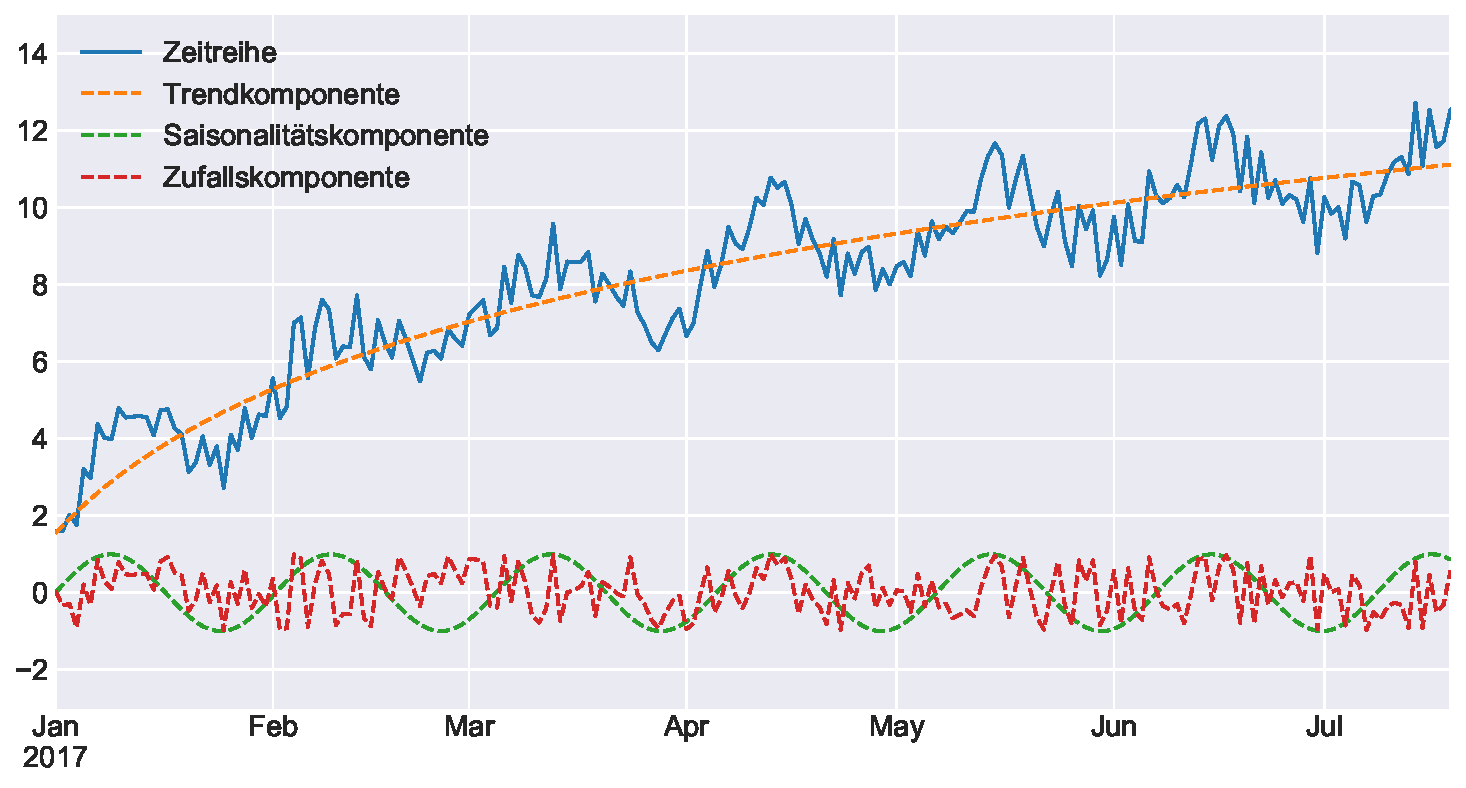
\includegraphics[width=\textwidth]{bilder/02-hauptteil/zeitreihe-komponenten.pdf}
  \caption[Aufteilung einer Zeitreihe in mehrere Komponenten]{Aufteilung einer Zeitreihe in mehrere Komponenten. Bild entnommen aus \citet{Masterthesis.2017}.}
  \label{fig:zeitreihe-komponenten}
\end{figure}
